\chapter{Preparation}
\label{chap:preparation}

\indent \indent
This chapter discusses the preparatory work done before beginning the project's implementation. §\ref{sec:preliminaries} introduces useful preliminary information and background, §\ref{sec:projectStrategy} discusses the methodologies used when approaching the design of the project's implementation, and §\ref{sec:startingPoint} provides an overview of the foundations of the project.

\section{Preliminaries}
\label{sec:preliminaries}
\setlength{\leftskip}{0.25cm}
\indent \indent
This section is dedicated to introducing the fundamental underlying concepts, terminologies, and notations fundamental to this project. The project spans two domains of computer science: cryptography and unsupervised machine learning. These are vast, active research areas. Therefore, for brevity, only concepts essential to understanding this dissertation will be presented - links to further resources may be provided for the sake of brevity.

\setlength{\leftskip}{0cm}

\subsection{Threat Model}
\label{sec:threatModel}
\setlength{\leftskip}{0.5cm}
\indent \indent
The design of this project considers the Machine Learning as a Service (MLaaS) framework, in which users first send their data to a server where machine learning inference is performed, and the results are returned. In particular, the transfer of surveillance video data to be analysed by security companies. Suppose that a subscriber to one of these services, Alice, sets up a camera to record activity at her front door. In this scenario, there are two critical threats: 
\begin{enumerate*}[label=$(\roman*)$]
    \item an adversary, Eve, may eavesdrop on the data while it is being transmitted between the client and server, and 
    \item an employee, Mallory, of the MLaaS provider may access the data while it is stored by the server, allowing them to monitor the activities of members of a household or observe the contents of a house, exposing risks of theft
\end{enumerate*}
Figure \ref{fig:threatModel} illustrates this succinctly. The first threat can be mitigated easily enough using cryptographic protocols such as TLS ~\cite{TLS}. However, the second threat is much more difficult to defend against, particularly because data must usually be decrypted for inference to be performed ~\cite{Bae}.
\smallskip \\ \indent
Fortunately, the use of HE can mitigate both of these risks. Firstly, HE is a secure cryptographic encryption scheme, so using it to encrypt data during transmission is sufficient to thwart eavesdropping adversaries. Secondly, HE allows computation to be performed on the data without decryption, so it can prevent the exploitation of plain data.

\begin{figure}[ht]
    \centering
    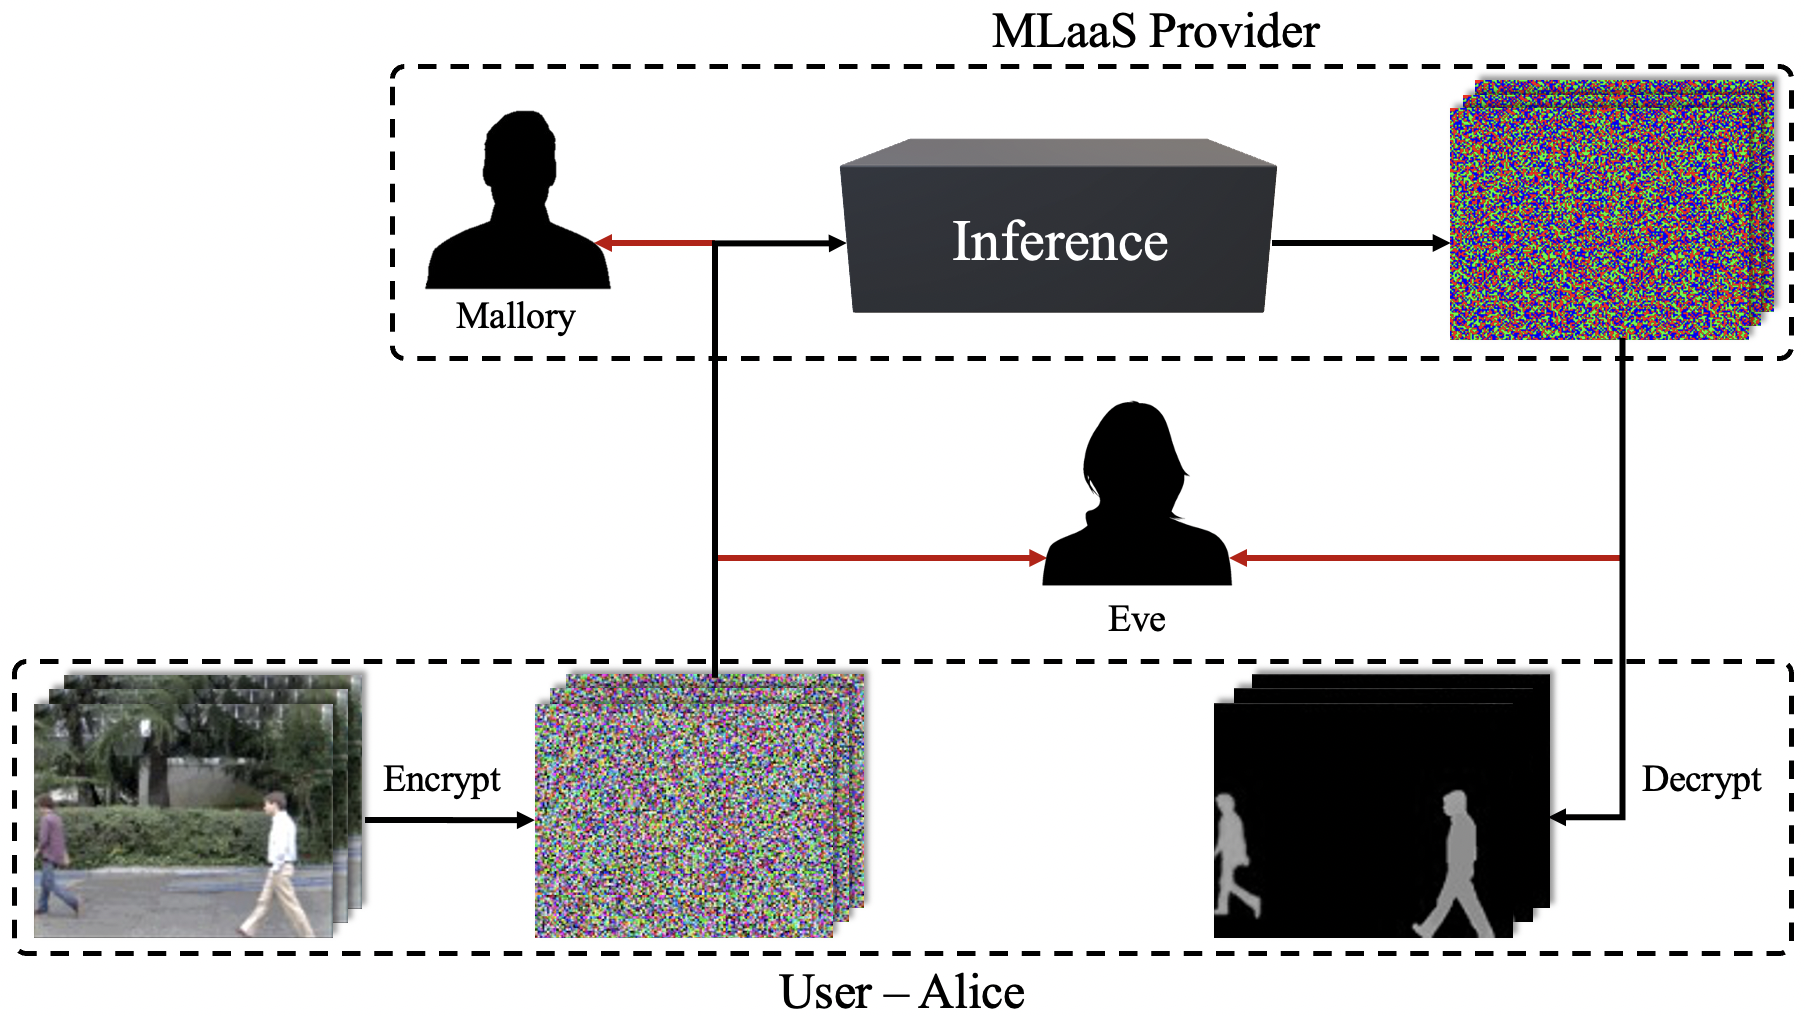
\includegraphics[width=0.9\textwidth]{figures/threatModel}
    \caption[The Threat Model]{A graphical representation of the threat model. Eve is an eavesdropper able to listen to communications between user an service provider. Mallory is a malicious individual within the service provider able to access users' video data. HE is able to obstruct both Eve and Mallory, preventing them from discovering the contents of the user's video.}
    \label{fig:threatModel}
\end{figure}

\setlength{\leftskip}{0cm}

\subsection{Homomorphic Encryption}
\label{sec:homomorphicEncryption}
\subsubsection{Introduction}
\setlength{\leftskip}{0.5cm}
\indent \indent
There are two broad categories of cryptographic encryption schemes: private-key (symmetric) and public-key (asymmetric). While both can be applied to HE, this dissertation will address public-key encryption because it is the technique adopted by all HE schemes used in the project.
\smallskip \\ \indent
A public-key encryption scheme is defined by a triple of functions $\Pi = (\texttt{KeyGen}, \texttt{Enc}, \texttt{Dec})$. \texttt{KeyGen} is a function used to generate a \textit{public key} (\texttt{PK}) and \textit{private key}\footnote{The \textit{private key} is referred to as a \textit{secret key} by some literature. While these terms are equivalent, general convention is to use \textit{secret key} in relation to symmetric encryption, and \textit{private key} when discussing asymmetric - a practice that this dissertation will follow.} (\texttt{SK}) such that $(\texttt{PK}, \texttt{SK}) \leftarrow \texttt{KeyGen}(1^l)$, where the security parameter, $l$, measures how hard it is for an adversary to break the scheme\footnote{An $l$-bit security parameter would require an expected $2^l$ attempts to guess the keys.}. Denoting the space of all possible plaintext messages as $\mathcal{M}$ and ciphertext messages as $\mathcal{C}$, a message $m \in \mathcal{M}$ is encrypted into its corresponding ciphertext $c \in \mathcal{C}$ by $c \leftarrow \texttt{Enc}_\texttt{PK}(m)$. Similarly $c$ is decrypted back into $m$ by $m \leftarrow \texttt{Dec}_\texttt{SK}(c)$.
\smallskip \\ \indent
In order to extend $\Pi$ into a HE scheme, a fourth function $\texttt{Eval}(f, c_1, \ldots, c_n)$ must be introduced. The evaluation function, $\texttt{Eval}$ applies a Boolean circuit, $f$, to the ciphertext arguments, $c1, \ldots, c_n$ such that, for all arguments, it holds that
\begin{equation}
    \texttt{Dec}_\texttt{SK}(\texttt{Eval}(f, c_1, \ldots, c_n)) = f(m_1, \ldots, m_n)
\end{equation}
where $m_1, \ldots, m_n$ are the plaintext equivalents of $c_1, \ldots, c_n$. This is, perhaps, better illustrated by Figure \ref{fig:homomorphicEncryption} below.

\begin{figure}[ht]
    \centering
    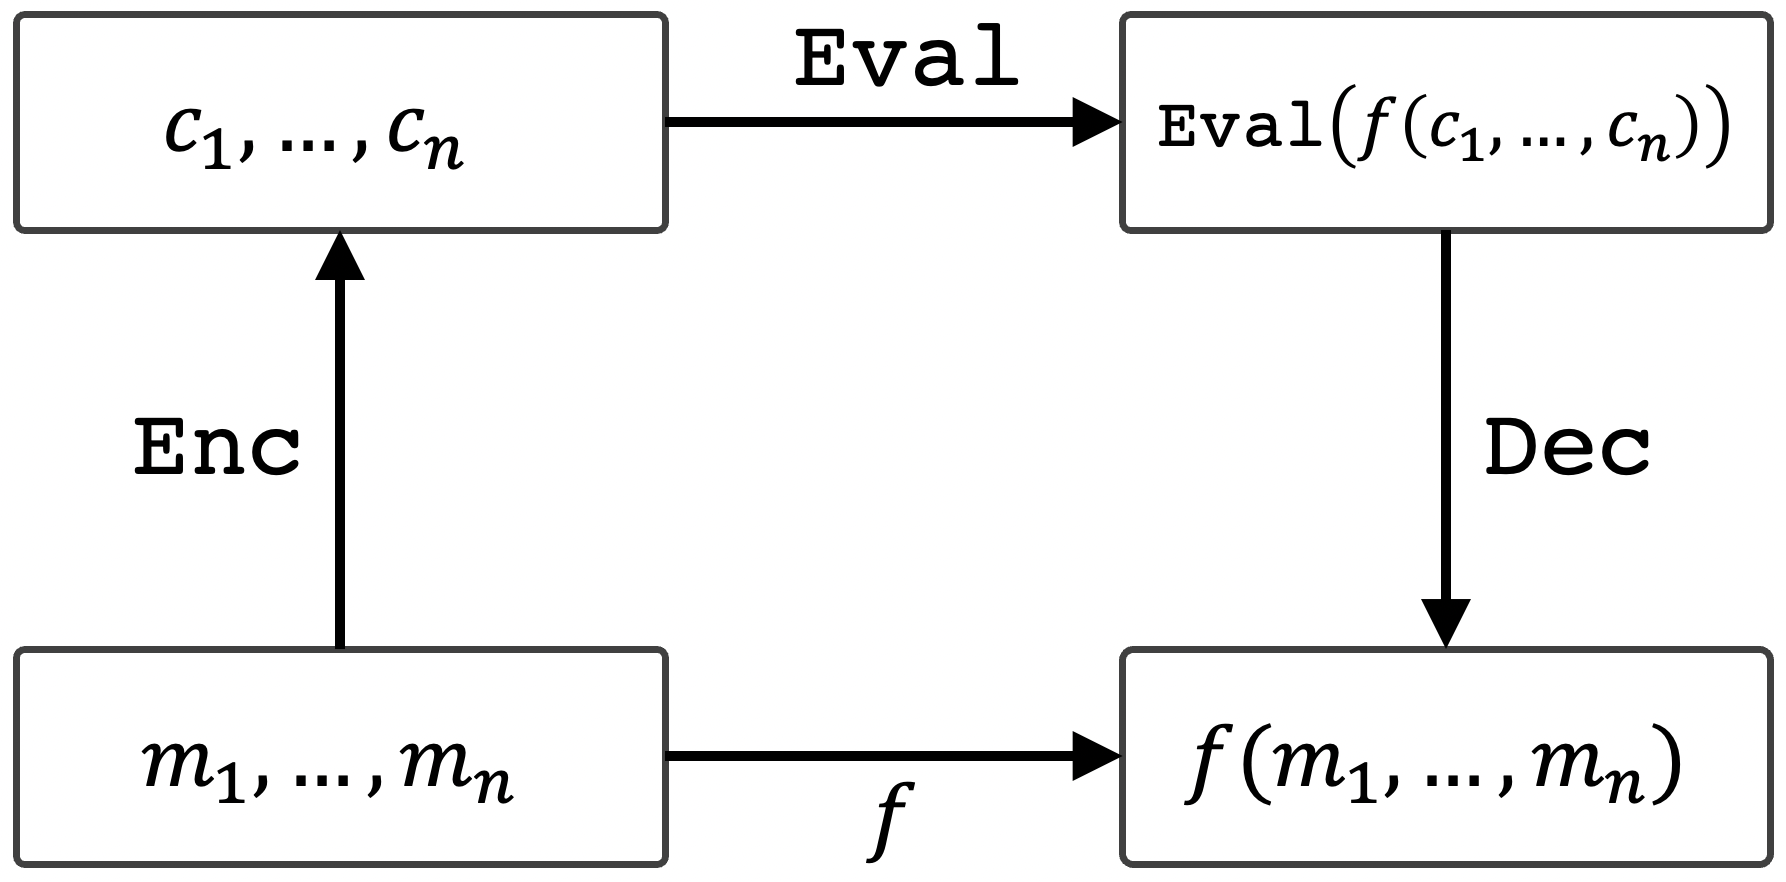
\includegraphics[width=0.6\textwidth]{figures/homomorphicEncryption.png}
    \caption[Homomorphic Encryption]{Homomorphic Encryption}
    \label{fig:homomorphicEncryption}
\end{figure}

Theoretically, a \textit{fully} homomorphic scheme\footnote{The prefix \textit{fully} derives from the existence of \textit{partially} homomorphic schemes. A partially homomorphic scheme will only allow certain operations on the ciphertext - usually multiplication and division - and have existed for many years. Some examples of partially homomorphic schemes include RSA, ElGamal, and Paillier encryption ~\cite{PartialSchemes}.} allows the evaluation of Boolean circuits indefinitely. However, in practice, the time complexity of operations means many schemes are \textit{levelled} homomorphic schemes. This means they only support operations up to a \textit{bounded depth} - that is, only a predefined number of circuits can be applied to a ciphertext before the plaintext becomes irrecoverable. The maximum depth is a critical factor when applying HE to practical problems because it significantly limits the scope of supported algorithms.

\setlength{\leftskip}{0cm}
\subsubsection*{Ring Learning with Errors}
\setlength{\leftskip}{0.5cm}
\indent \indent
For an encryption scheme to be \textit{perfectly secure}, a ciphertext must provide no additional information about its plaintext (see Equation \ref{eq:def1}). In other words, the probability of generating a given ciphertext from a particular plaintext is independent of the plaintext (see Equation \ref{eq:def2}). The two equations below can be shown to be equivalent using Bayes' rule. 
\begin{equation}
    \label{eq:def1}
    \probP(M = m \: | \: C = c) = \probP(C = c)
\end{equation}
\begin{equation}
    \label{eq:def2}
    \probP(C = c \: | \: M = m) = \probP(M = m)
\end{equation}
for all $m \in \mathcal{M}$, $c \in \mathcal{C}$.
\smallskip \\ \indent
While it is possible to create perfectly secure encryption schemes, they are impractical in real applications\footnote{For example, the One-Time Pad ~\cite{OTP}}. Therefore, \textit{computational security} is considered sufficient. Relying on the hardness of certain mathematical problems, computational security means that an encryption scheme is \textit{practically unbreakable}. That is, the most efficient known algorithm for breaking a cipher would require far more computational steps than an attacker would be able to perform, regardless of the hardware available to them. An example of this is the RSA encryption scheme which relies on the fact that there exists no known, efficient algorithm for computing the prime factors of a large number on a classical computer - the integer factorisation problem. In complexity theory, this problem falls into the set of $\mathcal{NP}$.
\smallskip \\ \indent
Similarly, the HE schemes used in this project rely on computational security rather than perfect security. More specifically, they utilise the hardness of the \textit{ring learning with errors} (henceforth RLWE) problem introduced by Lyubashevsky et al.\ ~\cite{RLWE}. A polynomial-time reduction from the \textit{shortest vector problem} to RLWE can be derived. Therefore, since the shortest vector problem is $\mathcal{NP}$-hard under the correct choice of parameters, it is safe to rely on RLWE for computational security.
\smallskip \\ \indent
RLWE considers the mathematical objects, \textit{rings}. To understand \textit{rings}, \textit{groups} must first be understood. A group $(\mathbb{G}, \bullet)$ is a set, $\mathbb{G}$, and an operator, $\bullet: \mathbb{G} \times \mathbb{G} \rightarrow \mathbb{G}$, such that the following properties hold:
\begin{itemize}
    \item \textbf{Closure}: $a \bullet b \in \mathbb{G}$ for all $a,b \in \mathbb{G}$.
    \item \textbf{Associativity}: $a \bullet (b \bullet c) = (a \bullet b) \bullet c$ for all $a, b, c \in \mathbb{G}$.
    \item \textbf{Neutral Element}: there exists an $e \in \mathbb{G}$ such that for all $a \in \mathbb{G}$, $a \bullet e = e \bullet a = a$
    \item \textbf{Inverse Element}: for each $a \in \mathbb{G}$ there exists some $b \in \mathbb{G}$ such that $a \bullet b = b \bullet a = e$
\end{itemize}
If $a \bullet b = b \bullet a$ for all $a, b \in \mathbb{G}$, the group is called \textbf{commutative} (or \textbf{abelian}). If there is no inverse element for each element, $(\mathbb{G}, \bullet)$ is a \textbf{monoid} instead.
\smallskip \\ \indent
From this, a \textit{ring} is defined as $(\textbf{R}, \boxplus, \boxtimes)$, where $\textbf{R}$ is a set, $\boxplus: \textbf{R} \times \textbf{R} \rightarrow \textbf{R}$, and $\boxtimes: \textbf{R} \times \textbf{R} \rightarrow \textbf{R}$, such that
\begin{itemize}
    \item $(\textbf{R}, \boxplus)$ is an abelian group.
    \item $(\textbf{R}, \boxtimes)$ is a monoid.
    \item $\boxplus$ and $\boxtimes$ are distributive - for all $a, b, c \in \textbf{R}$, $a \boxtimes (b \boxplus c) = (a \boxtimes b) \boxplus (a \boxtimes c)$ and $(a \boxplus b) \boxtimes c = (a \boxtimes c) \boxplus (b \boxtimes c)$.
\end{itemize}
If $a \boxtimes b = b \boxtimes a$ then it is a \textbf{commutative} ring, but this is not necessary for rings generally. One example of a ring is $(\mathbb{Z}[x], +, \times)$.
\smallskip \\ \indent
Specifically, the RLWE problem is concerned with the ring formed by the set of polynomials modulo $\Phi (X)$ that also have coefficients in $\mathbb{Z}_q$\footnote{$\mathbb{Z}_q$ is the set of integers modulo $q$. For example, $\mathbb{Z}_7 = \{0, 1, 2, 3, 4, 5, 6\}$.}. Known as a \textit{quotient ring}, this can be denoted by $\mathcal{R}_q = \mathbb{Z}[X] / (\Phi(X))$, where $\Phi(X)$ is an \textit{irreducible polynomial} - a polynomial which cannot be factored into two non-constant polynomials.
\smallskip \\ \indent
Informally, RLWE describes the problem of finding an unknown $s \in \mathcal{R}_q$ given a vector of polynomials computed using $s$ and some sampled errors. Consequently, an encryption scheme can be created such that, after encoding a plaintext vector, $\vec{v}$, as a list of polynomials and then using a secret polynomial to convert this list to a polynomial, it is infeasible to recover $\vec{v}$ in polynomial time.
\smallskip \\ \indent
The HE schemes discussed in this dissertation rely on the RLWE problem to assert \textit{indistinguishable encryptions under a chosen-plaintext attack} (IND-CPA) security. Fundamentally, any encryption scheme is IND-CPA secure if, when attacked by a probabilistic, polynomial-time adversary, the chances of correctly deciding which of two plaintexts a particular ciphertext corresponds to is even. Therefore, in practice, even if an adversary has access to an encryption \textit{oracle} that will encrypt any data an adversary provides, the adversary's chances of calculating the correct plaintext when given a ciphertext should be no better than if they were randomly guessing. 
\smallskip \\ \indent
Practically, HE schemes choose a \textit{cyclotonic polynomial} for $\Phi(X)$, where the $n$-th cyclotonic polynomial, $\Phi_n(X)$, is defined as
\begin{equation}
    \Phi_n(X) = \prod_{k \in [1, n]; \; gcd(k, n = 1)} X - e^\frac{2 i \pi k}{n}
\end{equation}
In order to speed up computation, $n$ is selected to be an even power of two. Consequently, $\Phi_n(X) = X^\frac{n}{2} + 1$. This allows the \textit{number theoretic transform} (NTT)\footnote{A specialisation of the discrete Fourier transform, the NTT is a generalisation of the Fast Fourier transform in the case of finite fields. ~\cite{NTT}}. The advantage of this is that it can be easily accelerated using hardware ~\cite{Hardware}.
\smallskip \\ \indent
The sampled errors used when deriving ciphertexts implies almost exponential growth in error in the number of multiplications applied. The limited depth property of levelled HE schemes is a direct result of this. However, the relative growth size can be reduced by increasing the modulus $q$. Although this is not without risks. If a polynomial degree of size $n/2$ is used, efficient attacks exist against the RLWE problem for a small value of $q$ ~\cite{HEStandard}. Therefore, a fundamental trade-off is introduced between the supported depth of multiplication and the security level.

\setlength{\leftskip}{0cm}




\subsection{Moving Object Detection}
\label{sec:movingObjectDetection}
\subsubsection{Introduction}
\setlength{\leftskip}{0.5cm}
\indent \indent
A discussion of \textit{image segmentation} has been well established in the fields of digital image processing and computer vision research. The problem describes the process of partitioning a digital image into multiple regions, represented as sets of pixels. The goal of segmentation is to simplify the representation of an image so that it is easier to analyse. For example, to locate objects, or boundaries, in an image. More precisely, image segmentation is the process of labelling each pixel of an image such that all pixels sharing a particular characteristic are assigned the same label ~\cite{Shapiro}.
\smallskip \\ \indent
There are two broad categories of segmentation techniques: \textit{semantic segmentation} and \textit{instance segmentation}. Semantic segmentation is an approach for grouping objects based on predefined categories. For example, all people in an image may be labelled as ``people'', all vehicles labelled ``vehicles'', and all animals labelled as ``animals'' ~\cite{Semantic}.  In contrast, instance segmentation provides a more refined categorisation of objects. This approach splits each category into separate occurrences. For example, each person in an image may be highlighted distinctly ~\cite{Instance}.
\smallskip \\ \indent
One application of image segmentation is \textit{foreground extraction}, also known as \textit{background subtraction}, which describes the techniques of segmenting an image into two groups: the foreground and the background, so that further processing can be applied. In order to perform background subtraction, the background of an image must be modelled so that changes in the scene can be detected. However, this can be difficult to achieve. Image data can be very diverse, with factors such as variable lighting, repetitive movements (like leaves, waves, and shadows) making robust models hard to develop.
\smallskip \\ \indent
Once a background subtraction model has been developed, it can be used to detect moving objects in videos. This is accomplished by comparing the foreground of the current frame to the foreground of a reference frame and extracting the observed differences. There are several methods for achieving this. Below are the five algorithms investigated for this dissertation.

\setlength{\leftskip}{0cm}
\subsubsection{Frame Differencing}
\setlength{\leftskip}{0.5cm}
\indent \indent
The most straightforward moving object detection algorithm, \textit{frame differencing} works by iterating through the frames of a video in a single pass. First, a reference frame must be established as the background. There are several options for this. One approach is to store the first frame of the video. Another, more common option is to compare each frame to the frame directly before it. The advantage of this is that it will evolve, so if a new object is permanently added to the scene, it won't be included in the foreground forever\footnote{For example, if a fence was added around someone's property or a car was parked in the scene, comparing to a static frame would mean these objects would always be highlighted by frame differencing, despite not moving}. However, there are disadvantages to this approach if an object is moving slowly enough to overlap with itself across frames. A balance can be found by periodically updating the reference frame or comparing each frame to one several before it, for example.
\smallskip \\ \indent
Each frame can be considered once the reference frame, $B$, has been selected. Denoting the frame at time $t$ as $f_t$, the value of each pixel in $B$, $P(B)$, can be subtracted from the corresponding pixel in $f_t$, $P(f_t)$. This can be represented mathematically by Equation \ref{eq:frameDifferencing}.
\begin{equation}
    \label{eq:frameDifferencing}
    P(F_t) = P(f_t) - P(B)
\end{equation}
where $F$ represents the frames in the resultant video highlighting moving objects.

\setlength{\leftskip}{0cm}
\subsubsection{Mean Filter}
\setlength{\leftskip}{0.5cm}
\indent \indent
A \textit{mean filter} approach to moving object detection attempts to overcome the weaknesses of selecting a reference frame when performing frame differencing. Instead of taking a frame directly from the video, the value of $B$ at time $t$ is calculated using Equation \ref{eq:meanFilter}.
\begin{equation}
    \label{eq:meanFilter}
    B = \frac{1}{N} \sum^N_{i=1} f_{t-i}
\end{equation}
where $N$ is the number of preceding images included in the average, and $f_t$ is the frame in the video at time $t$. $N$ would depend on the video speed and the amount of motion expected in the video.
\smallskip \\ \indent
After $B$ has been calculated at time $t$, the value of the resultant video $F_t$ can be calculated using the same method as frame differencing, given by Equation \ref{eq:frameDifferencing}.

\setlength{\leftskip}{0cm}
\subsubsection{Median Filter}
\setlength{\leftskip}{0.5cm}
\indent \indent
Performing moving object detection using a median filter is almost identical to the mean filter method. The difference arises in how the reference frame is calculated. In this approach, the median of the preceding $N$ frames is calculated instead of the mean.
\smallskip \\ \indent
Then, like the preceding methods, the moving objects are extracted by subtracting the reference frame from each frame in the video, according to Equation \ref{eq:frameDifferencing}.

\setlength{\leftskip}{0cm}
\subsubsection{Gaussian Average}
\setlength{\leftskip}{0.5cm}
\indent \indent
Wren et al.\ originally proposed fitting a Gaussian probabilistic density function to the most recent $N$ frames ~\cite{Wren}. Rather than storing a simple reference image that is subtracted from each frame in the video, this method stores a mean and variance value for each pixel in a video frame. The likelihood of a value of a particular pixel occurring can be calculated using this. It is assumed that the most likely value for a pixel will be equivalent to the background of a scene, so if an observed value is sufficiently unlikely according to its Gaussian distribution, it must be because a change has occurred in that portion of the frame. Therefore, that pixel is added to the foreground segment of the video.
\smallskip \\ \indent
A na\"ive approach to the Gaussian Average method would be to iterate through each frame in the video, calculating the mean and variance for each pixel and evaluating the likelihood from scratch every time. This would have quadratic complexity since, for each frame, $N$ calculations per pixel would have to be performed. A more efficient algorithm would utilise a cumulative function for the mean and standard deviation that can be updated in constant time. Consequently, this would have linear complexity because only a single calculation would need to be performed for each pixel in each frame. This approach would update the mean using Equation \ref{eq:mean}, and the variance using Equation \ref{eq:variance}.
\begin{equation}
    \label{eq:mean}
    \mu_t =
    \begin{cases}
        f_0 & \text{if $t = 0$} \\
        \alpha f_t + (1 - \alpha) \mu_{t-1} & \text{otherwise}
    \end{cases}
\end{equation}
\begin{equation}
    \label{eq:variance}
    \sigma^2_t =
    \begin{cases}
        c & \text{if $t = 0$} \\
        d^2 \alpha + (1 - \alpha) \sigma^2_{t-1} & \text{otherwise}
    \end{cases}
\end{equation}
where $\alpha$ determines the size of the \textit{temporal window} used to fit the Gaussian model\footnote{$\alpha$ acts similarly to a decay factor, weighting the most recent frames as more impactful on the model. Eventually, an old frame will be weighted so insignificantly that its impact is negligible. Therefore, it determines how far into the past the model uses to predict future pixels, hence the `temporal window'.}, $d = |f_t - \mu_t|$ gives the Euclidean distance from the pixel to the mean, and $c$ is some constant defined by the model creator. 
\smallskip \\ \indent
From these models, the foreground can be extracted according to Equation \ref{eq:meanThreshold},
\begin{equation}
    \label{eq:meanThreshold}
    \frac{|f_t - \mu_t|}{\sigma_t} > k
\end{equation}
where $k$ is a constant that the model creator can tune to achieve optimal results.
\smallskip \\ \indent
A variant of this method exists where the mean and variance are only updated if a pixel is believed to be in the background. This prevents the model from becoming skewed if there is lots of movement in the frame. However, it has severe limitations. For example, it only works if the image is initially entirely background, and it cannot cope with gradually changing backgrounds.

\setlength{\leftskip}{0cm}
\subsubsection{Gaussian Mixture Models}
\setlength{\leftskip}{0.5cm}
\indent \indent
Stauffer and Grimson proposed \textit{Gaussian mixture models} (henceforth GMMs) for moving object detection in 1999 ~\cite{Stauffer}. GMMs are probabilistic models that represent the presence of normally distributed subpopulations within an overall population. They are particularly useful because they don't require the subpopulation of a data point to be identified. Instead, subpopulations are learned automatically, constituting a form of unsupervised machine learning.
\smallskip \\ \indent
A simple application of GMMs is in modelling human heights. Typically, two Gaussian distributions will be used: one for males and one for females. Consequently, given just height data, with no gender assignments, it can be assumed that the distribution of all heights should follow the sum of two scaled and shifted Gaussian distributions. A model that can make this assumption on its own (or unsupervised) is an example of a GMM. In general, GMMs can be applied to more than two components.
\smallskip \\ \indent
There are two types of parameters necessary for GMMs, the \textit{component weights}, and the component \textit{means} and \textit{variances}. For a GMM with $N$ components, the $i^\text{th}$ component has $\mu_i$ and variance $\sigma_i$ in the \textit{univariate case}, and mean $\vec{\mu}_i$ and a covariance matrix $\Sigma_i$ in the \textit{multivariate case}. The component weights, $\phi_k$ for component $k$, are constrained by the equation $\sum^K_{i=1} \phi_i = 1$. If the component weights aren't learned, they are known as an \textit{a-priori}\footnote{A probability derived purely through deductive reasoning.} distribution over components such that $\probP(x \text{ generated by component k}) = \phi_k$. If the component weights are learned, they are known as \textit{a-posteriori}\footnote{From Bayesian statistics, referring to conditional probability $\probP(A | B)$.} estimates of the component probabilities given the data.
\smallskip \\ \indent
There are several methods for fitting the GMM's parameters. A common method is to use \textit{expectation maximisation} (EM), if the number of components of the GMM is known. When fitting a GMM, the Gaussian distributions are being tuned to match the distributions observed in the data. If all of the data is known, it can all be incorporated into this stage to achieve the most accurate fitting. However, in practice, it is likely that only a subset of the data will be available, so the GMM will then have to extrapolate to the real values. This technique can also be taken advantage of if there is limited time in which to perform fitting.
\smallskip \\ \indent
The EM algorithm is split into two many stages. Firstly, the E-step calculates the expectation of assigning each data point to each component of the GMM, given the GMM's parameters. Secondly, the M-step updates the values of each parameter to maximise the expectations. These two steps repeat until the algorithm converges. Informally, this works because knowing the component assignment for each data point makes solving for the parameters easy, and knowing the parameters makes inferring the probability of a component given the data point easy\footnote{The E-step corresponds to the latter case, and the M-step corresponds to the former.}. Therefore, by alternating which values are assumed known, maximum-likelihood estimates of the unknown values can be efficiently calculated.
\smallskip \\ \indent
Once a GMM has been fitted, it can be used for inference. There are two common uses of inference: \textit{density estimation} and \textit{clustering}. This dissertation will focus on clustering because it is most useful for moving object detection. The posterior component assignment probabilities can be estimated using Bayes' theorem combined with the GMM parameters. Knowing the component that a data point most likely belongs to provides a way to group the points into clusters. In the scenario of moving object detection, this would be two clusters: the foreground and the background.

\setlength{\leftskip}{0cm}





\section{Project Strategy}
\label{sec:projectStrategy}

\subsection{Requirements Analysis}
\label{sec:requirements}
\setlength{\leftskip}{0.5cm}
\indent \indent
The requirements for this project are listed below. The nature of the project required the development of theoretical knowledge before implementation began, and, as such, the requirements subtly evolved as understanding matured. The original requirements are given in Appendix \ref{app:proposal} for comparison. The final requirements have been grouped into two categories. The first, labelled $A$, are the core requirements deemed essential to the project's success. The second, labelled $B$, are considered extensions, aiming to improve understanding of the components used in the core implementation or further the investigation into the applications of HE in surveillance.
\subsubsection{Core}
\begin{enumerate}[leftmargin=1.75cm,label=\texttt{A\arabic*:}]
    \item \textit{Implement a client-server application allowing videos to be homomorphically encrypted and transmitted in both directions.} \smallskip \\ This component is vital because it provides the foundation for implementing and integrating all other components. It is also essential to emulate the MLaaS software stack. While conceptually simple, the nature of HE data adds many challenges to transferring videos, forming a significant portion of the investigation into HE applicability.
    \item \textit{Implement background subtraction models that can extract moving objects from homomorphically encrypted videos.} \smallskip \\ This requires designing and implementing the five moving object detection algorithms detailed in §\ref{sec:movingObjectDetection} so that they can act on HE data.
    \item \textit{Evaluate the accuracy of HE inference to investigate its applicability to real systems.} \smallskip \\ This involves analysing different metrics to understand the efficacy of moving object detection on HE data. Comparisons can be made between inference methods and between plain and encrypted data.
\end{enumerate}
\subsubsection{Extensions}
\begin{enumerate}[leftmargin=1.75cm,label=\texttt{B\arabic*:}]
    \item \textit{Implement a bespoke HE scheme and integrate it into the core application, providing the same functionality as the established scheme already used.} \smallskip \\ While this implementation will likely have worse performance than existing implementations, it will offer helpful insight into the inner workings of HE. Also, it may provide opportunities for optimisations for this specific application.
    \item \textit{Analyse the security of the encryption schemes used in the project.} \smallskip \\ This will be useful in ensuring HE can overcome both security and privacy concerns of existing surveillance solutions and doesn't accidentally introduce insecurities that could allow adversaries to extract information.
    \item \textit{Implement an object recognition algorithm acting on HE data using neural networks.} \smallskip \\ Implementations like Cryptonets \cite{Dowlin} have demonstrated the application of neural networks to HE. This would allow further services offered by surveillance companies to be emulated and reveal a greater insight into the limitations of HE in video analysis.    
\end{enumerate}

\setlength{\leftskip}{0cm}

\subsection{Methodology}
\setlength{\leftskip}{0.5cm}
\indent \indent
The different stages of the project were best suited to different development methodologies. For the core components, a waterfall development methodology was adopted ~\cite{Waterfall}. The requirements were detailed and unambiguous, so the project lent itself to a structured methodology, not requiring the flexibility of an iterative approach. The stages of the model are detailed below.
\begin{figure}[ht]
    \centering
    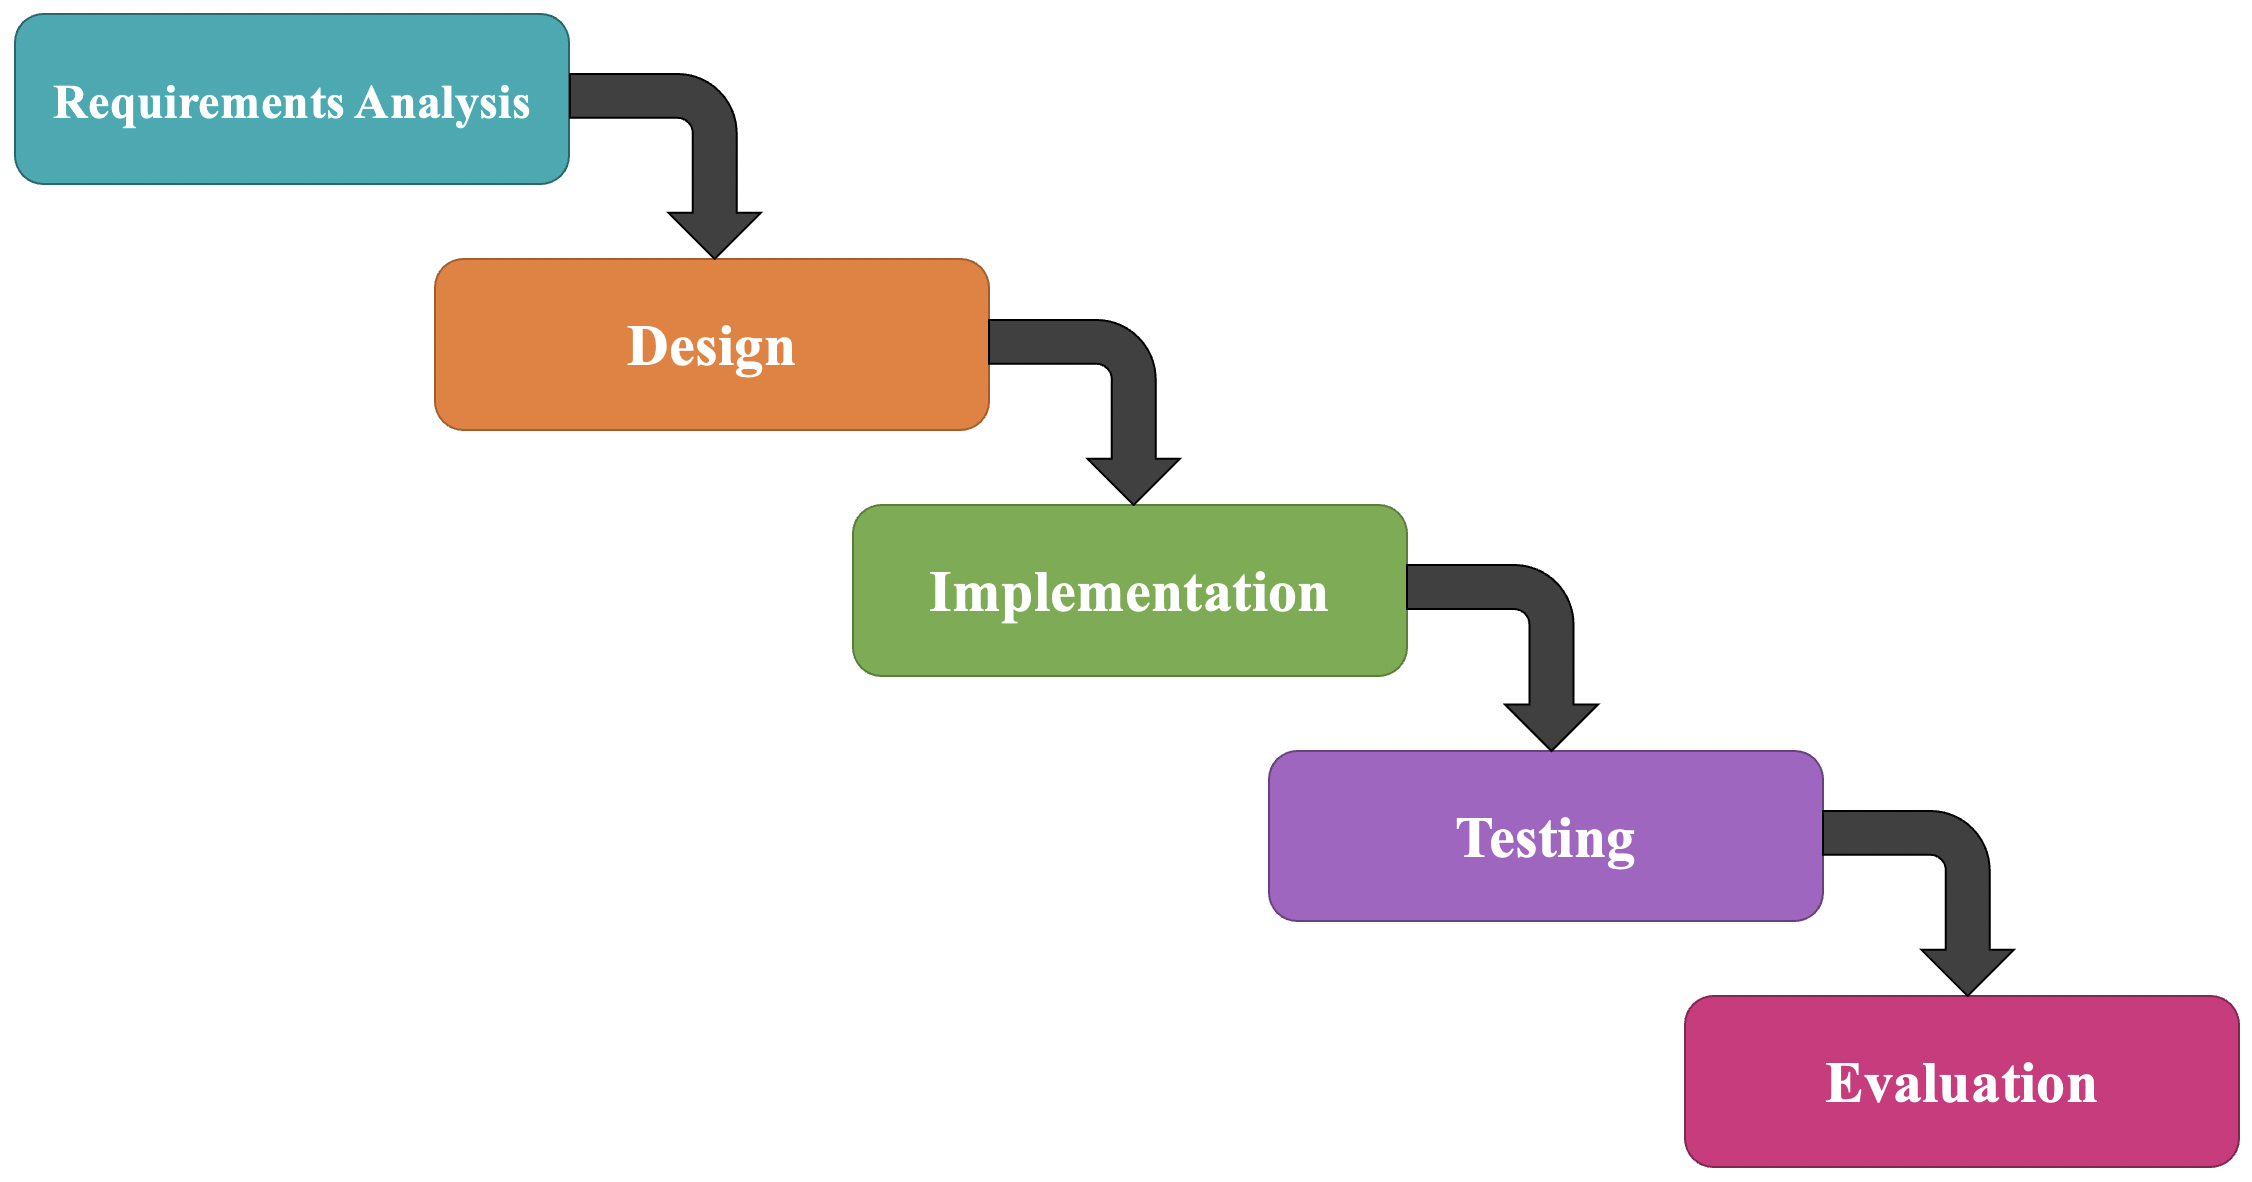
\includegraphics[width=0.8\textwidth]{figures/waterfall.png}
    \caption{The Waterfall Development Model}
    \label{fig:waterfall}
\end{figure}
\\ \indent
The results of the \textit{requirements analysis} stage have been detailed in §\ref{sec:requirements}. This stage is where most of the research was performed so that the project's design would be better informed.
\smallskip \\ \indent
The \textit{design} phase incorporates expanding on the requirements into a physical project; this includes, for example, creating the class diagrams shown in Figure \ref{fig:clientUML}, Figure \ref{fig:serverUML}, and Figure \ref{fig:mekksUML}.
\smallskip \\ \indent
The \textit{implementation} and \textit{testing} stages were intertwined where possible in order to promote a test-driven approach to development. This was made easier by the object-oriented methodology and unit testing practices (see §\ref{sec:testing}) adopted during the design stage.
\smallskip \\ \indent
The \textit{evaluation} stage replaces the \textit{maintenance} stage of the traditional Waterfall model because it is unsuitable for this project. This stage involves running experiments to evaluate the project.
\smallskip \\ \indent
When working on the extensions, an iterative model was more appropriate. For example, extension \texttt{B1} could be easily split into distinct modules, so they could be developed then tested in a repeating process. Therefore, development transitioned to an Agile model, depicted in Figure \ref{fig:agile}.
\begin{figure}[ht]
    \centering
    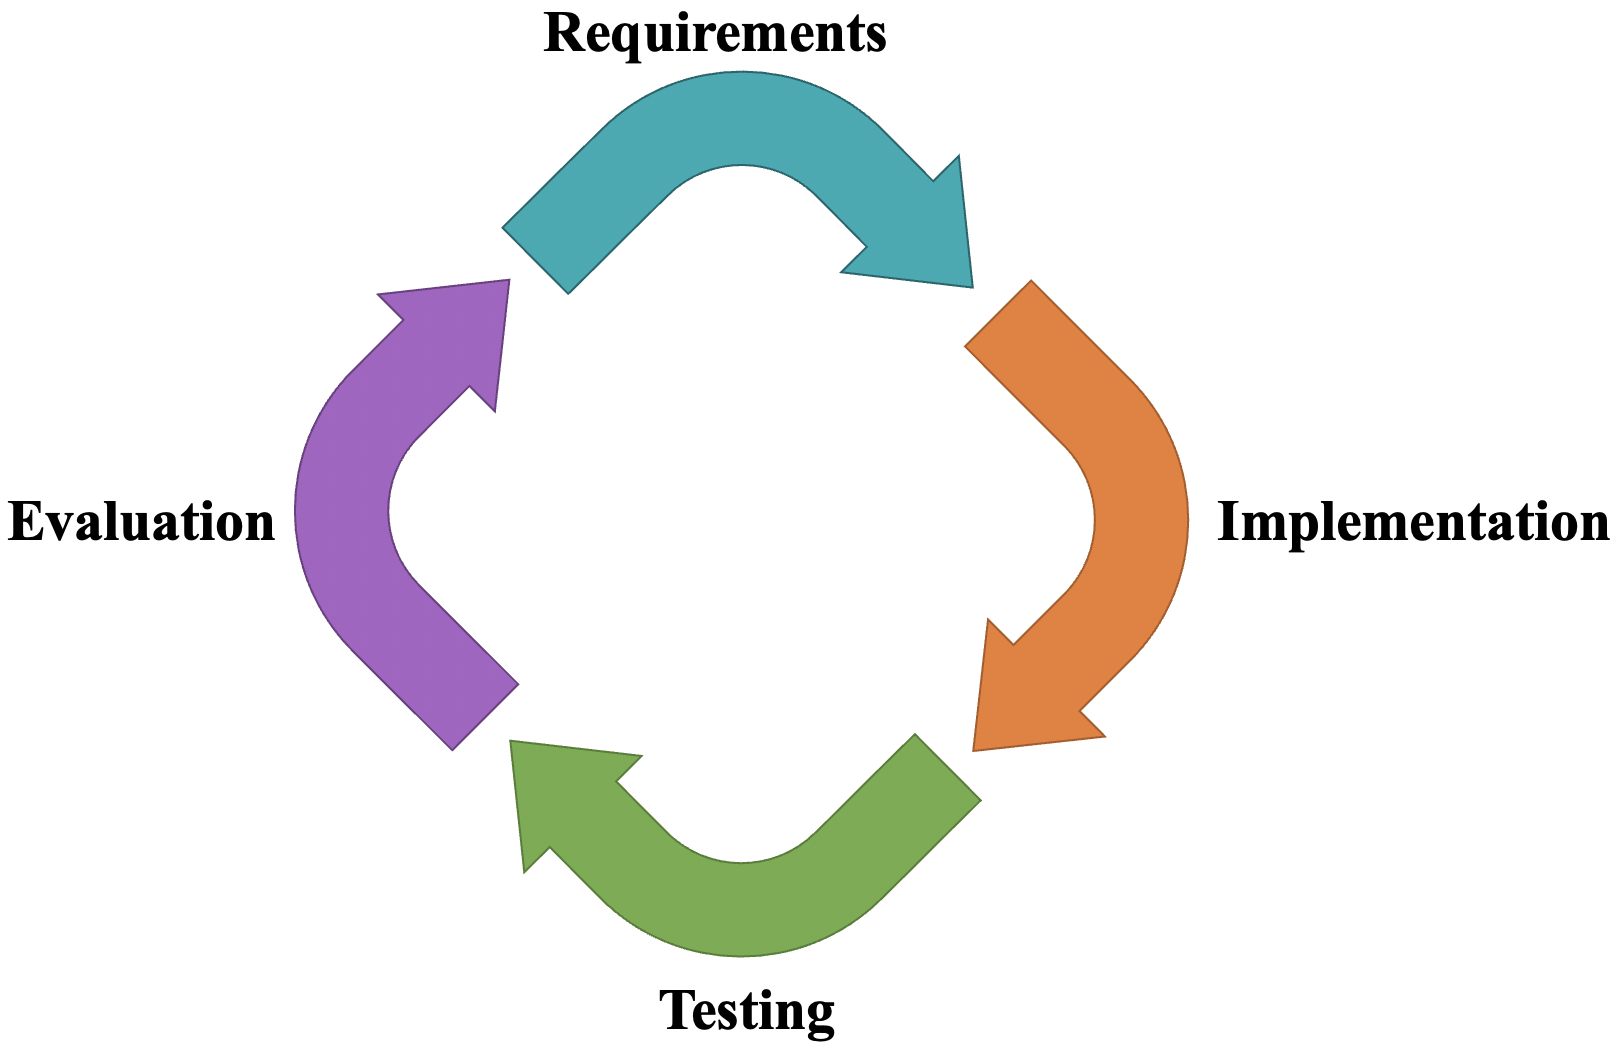
\includegraphics[width=0.6\textwidth]{figures/agile.png}
    \caption{The Agile Development Model}
    \label{fig:agile}
\end{figure}
\\ \indent
A Gantt chart of the project's timeline is shown in Figure \ref{fig:gantt}.
\begin{figure}[H]
    \centering
    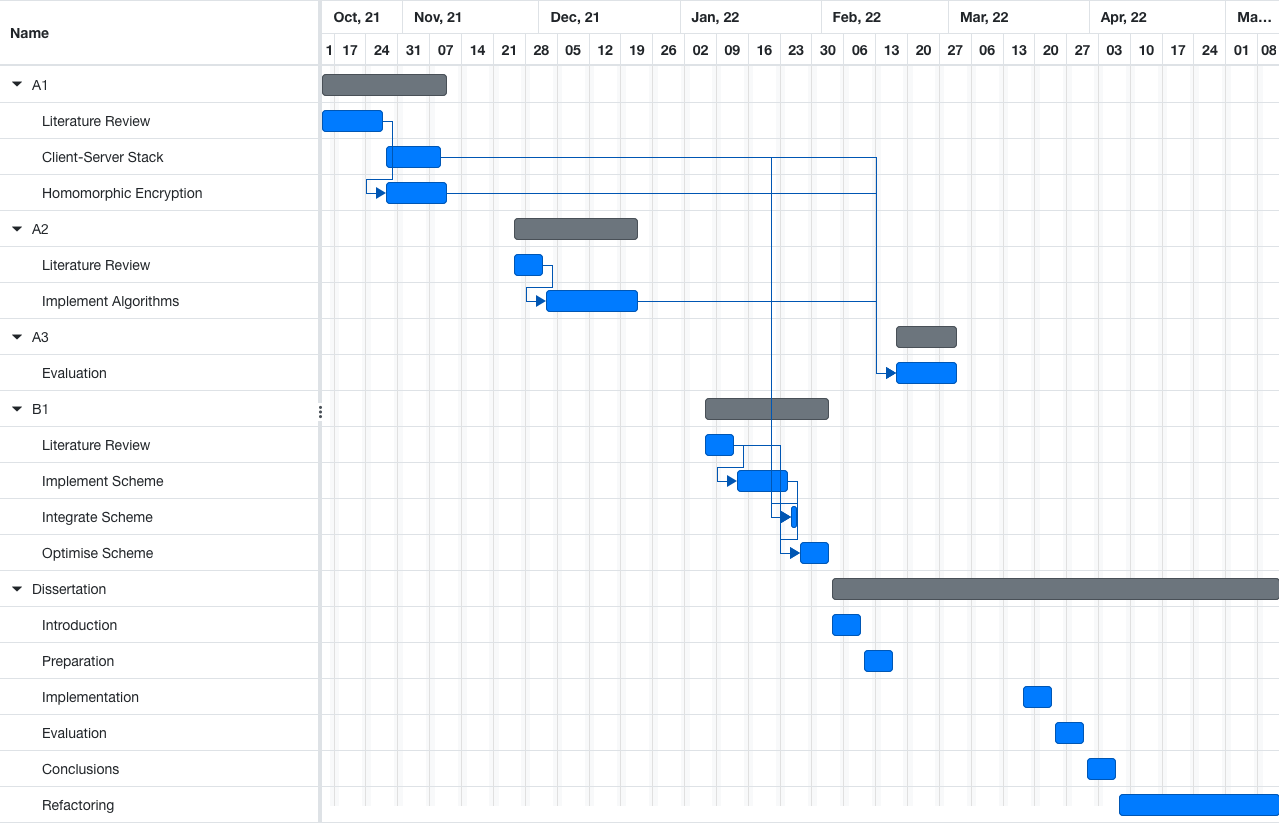
\includegraphics[width=1\textwidth]{figures/gantt.png}
    \caption{Project Timeline}
    \label{fig:gantt}
\end{figure}


\setlength{\leftskip}{0cm}

\subsection{Testing}
\label{sec:testing}
\subsubsection{Challenges}
\setlength{\leftskip}{0.5cm}
\indent \indent
Unlike traditional software engineering, machine learning does not provide precise criteria against which the correctness of an implementation can be verified. The models used for background subtraction are probabilistic, so the outputs cannot be precisely predicted.  Consequently, a variety of testing methodologies were required.

\setlength{\leftskip}{0cm}
\subsubsection{Unit Tests}
\setlength{\leftskip}{0.5cm}
\indent \indent
Designed for testing atomic units of source code, unit testing takes advantage of the independent nature of components written following object-oriented principles to test functions in isolation. It does this by providing known expected, boundary, and erroneous data and ensuring the results of a function match the expected. Unit tests can be automated, making them easy to run repeatedly as changes to the source code are made, ensuring errors aren't introduced.
\smallskip \\ \indent
Unit tests were particularly useful when developing a HE scheme from scratch. They verified the correctness of the encoding, encryption, and decryption functions and the HE Boolean circuits automatically and repeatedly.

\setlength{\leftskip}{0cm}
\subsubsection{Integration Tests}
\setlength{\leftskip}{0.5cm}
\indent \indent
While similar to unit tests, integration tests increase the scope of functionality covered by each test. The goal of integration testing is to ensure separate modules interact correctly. Once unit testing has been completed, these tests take the verified modules, group them into larger aggregates, and provide expected, boundary, erroneous data to ensure the output is correct.
\smallskip \\ \indent
Integration testing was useful in verifying that the software stack functioned correctly. For example, ensuring the client and server communicated correctly. While some integration testing can be automated, more complex engineering work was prioritised over creating a more comprehensive testing suite, so manual integration testing was the primary technique used.

\setlength{\leftskip}{0cm}
\subsubsection{Manual Verification}
\setlength{\leftskip}{0.5cm}
\indent \indent
Manual verification was used to overcome the challenges of testing the background subtraction models. Since the project involves video data, human inspection provides a good intuition of whether or not a background has been correctly removed. If a more detailed analysis is required, pixel values can be compared to check for expected results, or verify consistency across multiple tests\footnote{While humans are able to perform this verification, simple Python scripts are usually written to make testing more efficient.}. 

\setlength{\leftskip}{0cm}





\section{Starting Point}
\label{sec:startingPoint}

\subsection{Knowledge and Experience}
\setlength{\leftskip}{0.5cm}
\indent \indent
Prior to beginning the project, the following Tripos courses that considered similar themes had been completed: \textit{Scientific Computing}, \textit{Machine Learning and Real-world Data}, \textit{Software and Security Engineering}, \textit{Concurrent and Distributed Systems}, \textit{Data Science}, \textit{Computer Networking}, and \textit{Security}. The Part II course, \textit{Cryptography} was also useful in understanding the theoretical underpinnings of encryption.
\smallskip \\ \indent
However, it should be noted that HE is not included in the scope of the Cryptography course, so the theory was learned independently of Tripos studies. The study of applied HE is sparsely documented, particularly with modern schemes. Therefore, most understanding came from academic papers; notably \cite{CKKS} and \cite{SEAL}. Although, articles such as \cite{BrilliantHE} were more useful for foundational knowledge.
\smallskip \\ \indent
Similarly, there was little mention of computer vision artificial intelligence in Tripos, so most understanding came from independent research. For example, academic papers such as \cite{Stauffer} and \cite{Kulchandani} were helpful, particularly when considering privacy-preserving computer vision. Some understanding also came during a summer internship completed in the field of object recognition deep learning.

\setlength{\leftskip}{0cm}

\subsection{Tools Used}
\subsubsection{Programming Languages}
\setlength{\leftskip}{0.5cm}
\indent \indent
All of the code written for this dissertation was written in \textit{Python} ~\cite{Python}.  The main reasons for this were the large machine learning ecosystem, ease of use, and ease of debugging. Consequently, it was best suited to the project's tight schedule since it should allow for quick implementation.
\smallskip \\ \indent
However, it must be acknowledged that Python is not a language traditionally used for cryptographic applications. Usually, lower-level, faster languages like C++ are favoured. Since the original focus of the project was investigating the efficacy of moving object detection in the HE domain, the speed of execution was not prioritised over the speed of implementation.

\setlength{\leftskip}{0cm}
\subsubsection{Software Development}
\setlength{\leftskip}{0.5cm}
\indent \indent
\textit{Visual Studio Code} \cite{VSCode} development environment was used for writing code because of support for Python as well as a wide variety of plugins that allow integration of other valuable tools such as ESLint.  In addition, \textit{Git} \cite{Git} and \textit{GitHub} \cite{Github} were used for version control and source code management, as well as storing a backup of source code. \textit{OneDrive} \cite{OneDrive} was also used to hold another backup, for safety.

\setlength{\leftskip}{0cm}
\subsubsection{Encryption Schemes}
\setlength{\leftskip}{0.5cm}
\indent \indent
The project focuses on HE schemes based on the RLWE problem. The main reason for this was the abundance of academic literature discussing them. In particular, the CKK scheme \cite{CKKS} was selected because it supports representing real numbers\footnote{As opposed to, for example, the BFV scheme, which only supports integers ~\cite{BFV1, BFV2}.}. However, the project is designed in such a way that any HE encryption scheme can be substituted in CKKS's place, as long as it follows the same API.

\setlength{\leftskip}{0cm}
\subsubsection{Libraries}
\setlength{\leftskip}{0.5cm}
\indent \indent
The project uses Microsoft's SEAL library \cite{SEAL}, which provides a C++ implementation of the CKKS scheme. This was chosen because of the extensive optimisations that have been applied. In particular, SEAL uses a residue-number-system variant of CKKS to support large plaintext moduli. The SEAL API was integrated using a Python wrapper library ~\cite{Wrapper}.

\setlength{\leftskip}{0cm}
\subsubsection{Datasets}
\setlength{\leftskip}{0.5cm}
\indent \indent
There were two publicly available datasets used in this project:
\begin{itemize}[leftmargin=1.5cm]
    \item The Moving-MNIST dataset contains ten thousand sequences each of length twenty frames showing two handwritten digits from the standard MNIST dataset moving in a $64 \times 64$ pixel frame. This is a relatively simple dataset to perform moving object detection on because it only contains white objects on a black background. Therefore, it was useful in providing a baseline for the performance of the inference algorithms. \cite{MovingMNIST, MNIST}.
    \item The LASIESTA dataset contains a variety of sequences showing objects moving across static backgrounds in a range of conditions. Specifically designed to evaluate segmentation algorithms, this dataset provides a more realistic example of surveillance video. Therefore, this dataset can provide a truer evaluation of moving object detection in the HE domain. \cite{LASIESTA}.
\end{itemize}

\setlength{\leftskip}{0cm}
\subsubsection{Licensing}
\setlength{\leftskip}{0.5cm}
\indent \indent
All software dependencies in this project use permissive libraries that allow their code to be used without restrictions. The same is true for the datasets. Table \ref{tab:licensing} gives the specific licenses.
\begin{table}[H]
\centering
\def\arraystretch{1.25}
\begin{tabular}{|p{5cm}|p{4cm}|}
    \hline
    \textrm{\textbf{Dependency}} & \textrm{\textbf{Licence}} \\
    \hline \hline
    \texttt{Multiprocessing} & \multirow{3}{*}{\textrm{3-Clause BSD ~\cite{BSD}}} \\ 
    \texttt{NumPy} & \\ 
    \texttt{SymPy} & \\
    \hline
    \texttt{Microsoft SEAL} & \multirow{2}{*}{\textrm{MIT ~\cite{MIT}}} \\
    \texttt{SEAL-Python} & \\
    \hline
    \texttt{Matplotlib} & \multirow{3}{*}{\textrm{PSFL ~\cite{PSFL}}} \\ 
    \texttt{Python} & \\
    \texttt{Tkinter} & \\
    \hline
\end{tabular}
\caption{Licenses}
\label{tab:licensing}
\end{table}

\setlength{\leftskip}{0cm}

\subsection{Computer Resources}
\setlength{\leftskip}{0.5cm}
\indent \indent
The original project proposal mentioned that external computational resources might have been required during the implementation phase, such as AWS or Microsoft Azure. However, the project was entirely developed, tested, and evaluated on a MacBook Pro laptop. The specifications are listed below, in Table \ref{tab:specs}.
\\
\begin{table}[H]
\centering
\begin{tabular}{>{\hspace{1em}}l l}
    \myheading{\textrm{Processor}}
    \textrm{CPU}                       & \SI{8}{\; Cores}                                            \\
    \textrm{GPU}                       & \SI{14}{\; Cores}                                           \\
    \textrm{Neural Engine}             & \SI{16}{\; Cores}                                           \\
    \textrm{Memory Bandwidth}          & \SI{200}{\; GB \per s}                                      \\
    \myheading{\textrm{Memory}}
    \textrm{RAM}                       & \SI{32}{\; GB \text{ (unified memory)}}                     \\
\end{tabular}
\caption{Computer Specifications}
\label{tab:specs}
\end{table}

\setlength{\leftskip}{0cm}
